\documentclass[11pt,a4paper]{article}
\usepackage{amsmath}               % To include equation enviroment
\usepackage{graphicx}              % To include graphics enviroment
\usepackage[margin=1in]{geometry}  % Package to modify page layout, setting margin size
\usepackage[round]{natbib}         % Used for citation style to read author and year as oppose to number
\usepackage{tabularray}            % A nicer package, than the inbuilt, for the definition of tables
\usepackage{fancyhdr}              % Customise the header and footer
\usepackage{siunitx}               % Package for standarised SI units


% === === === Inline Bibilography === === ===
\begin{filecontents}[overwrite]{biblio.bib}

@Book{Leishman,
author = {Leishman},
title = {Principles of Helicopter Aerodynamics},
publisher = {Cambridge Aerospace Series},
year = {2006},
edition = {2nd}
}



\end{filecontents} 



% === === === Main Document === === ===
\begin{document}

\setlength{\parindent}{0cm}

% Setup some macros for setting variables used multiple times
\newcommand{\Issue}{1.0}
\newcommand{\Date}{Feb 2024}
\newcommand{\Equation}[1]{equation (\ref{#1})}

% Setup header and footer styles
\fancypagestyle{firstpagestyle}
{
   \fancyhf{}
   \pagestyle{fancy}
	\fancyhead{} % Clear the header
	\setlength{\headheight}{33.0pt}
	\fancyhead[R]{
\includegraphics[height=1cm]{ArduPilot_logo.jpg}} % Add AP logo
	\renewcommand{\headrulewidth}{0pt} % Remove the line
	\fancyfoot{} % Clear the footer
	\fancyfoot[L]{\large Issue \Issue}
	\fancyfoot[C]{\large Page \thepage}
	\fancyfoot[R]{\large \Date}
}

\fancypagestyle{otherpagestyle}
{
   \fancyhf{}
   \pagestyle{fancy}
	\fancyhead{} % Clear the header
	\renewcommand{\headrulewidth}{0.5pt}
	\setlength{\headheight}{33.0pt}
	\fancyhead[R]{
\includegraphics[height=1cm]{ArduPilot_logo.jpg}} % Add AP logo
	\fancyhead[L]{\large \textbf{Derivation of Autonomous\\Autorotation Equations}}
	\fancyfoot{} % Clear the footer
	\fancyfoot[L]{\large Issue \Issue}
	\fancyfoot[C]{\large Page \thepage}
	\fancyfoot[R]{\large \Date}
}

% Set the first page style
\thispagestyle{firstpagestyle}


% --- Title ---
\begin{center}
{\Large \textbf{Derivation of Equations used in ArduPilots Autonomous Autorotation Flight Mode}}\\[1.6cm]
\end{center}


\section{Introduction}

This short report gives an overview of the equations used within the autonomous autorotation flight mode implimented in ArduPilot, for use with traditional helicopters.

The purpose of this document is to provide a guide to developers, giving the derivation of the equations used, making the code implementation easier to follow, and preserving the intent and rational as to why the controller is written as it is.

In an attempt to keep this document brief, where possible, equations from other resources have been used as a starting point, to avoid duplication of already available and well documented methods.  All references and links are provided.


\section{Nomenclature}

\begin{table}[h!]
    \centering
    \begin{tblr}{
    			colspec={Q[c,m]Q[l,m]},
    			column{1}={2.0cm},
    			%column{2}={1.25cm},
    			}
		$C_{l_{\alpha}}$    &  (\unit{\per\radian}) lift-curve slope.  \\
		$r$                 &  Non-dimensional radial distance.  \\
    	$\lambda$           &  Rotor inflow ratio (normalised by tip speed).  \\
    	$\lambda_{i}$       &  Induced inflow ratio.  \\
    	$\lambda_{h}$       &  Induced inflow ratio in the hover.  \\
    	$\lambda_{c}$       &  Climb inflow ratio.  \\
    	$\sigma$            &  Rotor solidity ratio.  \\
    	$\theta$            &  (\unit{\radian}) Blade pitch angle.  \\
	\end{tblr}
\end{table}

TODO: Add a few diagrams of rotor geometry to help introduce the nomenclature.


\section{Flare Hight Estimate}

In order to approximate what height the aircraft will begin to flare, Blade Element Momentum Theory (BEMT) is used to construct an approximation of the decceleration that can be expected from the helicopter in the flare, hence at what height the flare must begin to achieve a successful landing

TODO: Give a little flow diagram of the calculation order to provide context

\subsection{Approximation of Hover Inflow Ratio}

Starting from equation (3.60) of \cite{Leishman} (Page 127), the local rotor inflow ratio ($\lambda$) that is a function of the non-dimensional rotor radius ($r$), $\lambda = \lambda(r)$, can be computed from the following quadratic:

\begin{equation}
	\label{eq:InflowQuad}
	\lambda^{2} + \left(\dfrac{\sigma \; C_{l_{\alpha}}}{8} - \lambda_{c} \right) - \dfrac{\sigma \; C_{l_{\alpha}}}{8} \; \theta \; r = 0
\end{equation}

For cleanliness in the equations, the solidity ratio ($sigma$) and lift-curve slope ($C_{l_{\alpha}}$) are grouped into one variable $b = \sigma \; C_{l_{\alpha}}$, giving:

% Page breaks here go to new page style
\newpage
\thispagestyle{otherpagestyle}

\begin{equation}
	\lambda^{2} + \left(\dfrac{b}{8} - \lambda_{c} \right)\lambda - \dfrac{b}{8} \; \theta \; r = 0
\end{equation}

In this application the hover case is of specific interest, hence the induced flow ratio in the hover ($\lambda_{h}$) can be obtained by setting $\lambda_{c} = 0$, and recalling that the definition of $\lambda = \lambda_{i} + \lambda_{c}$, thus:

\begin{alignat}{2}
	\lambda_{h} = \lambda_{i} = \lambda - \lambda_{c} &= \lambda, \notag \\
    \lambda_{h}^{2} + \dfrac{b}{8}\lambda_{h} - \dfrac{b}{8} \; \theta \; r & = 0 \label{eq:HoverInflow}
\end{alignat}

Solving for the roots of the quadratic in \Equation{eq:HoverInflow} to obtain:

\begin{alignat}{2}
	\lambda_{h} &= \dfrac{1}{2} \left( - \dfrac{b}{8} \pm \sqrt{\left(\dfrac{b}{8}\right)^{2} + 4 \; \dfrac{b}{8} \; \theta \; r } \right) \notag \\
	\lambda_{h} &= - \dfrac{b}{16} \pm \sqrt{\dfrac{b^{2}}{256} + \dfrac{b}{8} \; \theta \; r }
\end{alignat}



\begin{figure}[h!]
	\centering
	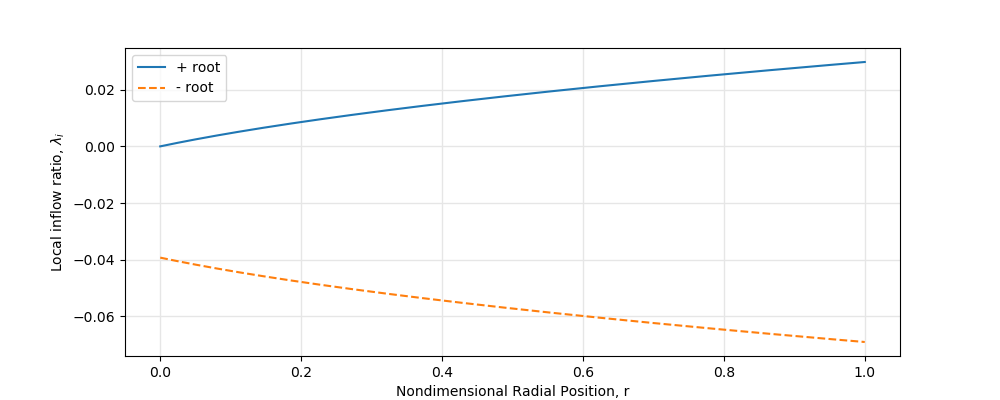
\includegraphics[width=\textwidth]{inflow_distribution.png}
	\caption{Local inflow distribution obtained by the roots of equation \ref{eq:InflowQuad}.\label{fig:InflowDist}}
\end{figure}





% --- References ---
\renewcommand{\bibname}{References}
\bibliographystyle{plainnat}
\bibliography{biblio}

\end{document}
